\documentclass{beamer}
%\usepackage[MeX]{polski}
%\usepackage[cp1250]{inputenc}
\usepackage{polski}
\usepackage[utf8]{inputenc}
\title{Stadion Narodowy w Warszawie}
\author{Michał Samsel}
\date{\today}
\institute{UWM}
\beamersetaveragebackground{blue!10}
\usetheme{Warsaw}
\usecolortheme[rgb={0.1,0.5,0.7}]{structure}
\usepackage{beamerthemesplit}
\usepackage{multirow}
\usepackage{multicol}
\usepackage{array}
\usepackage{graphicx}
\usepackage{enumerate}
\usepackage{amsmath} %pakiet matematyczny
\usepackage{amssymb} %pakiet dodatkowych symboli

%opening
\begin{document}
	\frame{\titlepage}

	\begin{frame}
		\frametitle{Spis Treści}
		\tableofcontents
	\end{frame}

	\section{Ogólnie o stadionie}
	\begin{frame}{Stadion liczbowo}
		\begin{itemize}
		\item Data otwarcia: 29 stycznia 2012
		\item Inauguracja: 29 lutego 2012 Polska – Portugalia 0:0
		\item Pojemność: 58 500 (mecze)
		\item Wymiary: 105m x 68m
		\end{itemize}
	\end{frame}
	
	\begin{frame}{Cel stadionu}
	Stadion zbudowano z myślą o piłkarskich Mistrzostwach Europy 2012. Stadion jest wielofunkcyjnym obiektem sportowym  umożliwiającym organizacje wydarzeń sportowych, kulturalnych lub koncertów muzycznych.
	\end{frame}
	
	\section{Wyposażenie stadionu}
	\begin{frame}{Płyta i murawa}
	Powierzchnia jest trawiasta. Obiekt posiadana podgzewaną płytę boiska. Początkowy plan zakładał modułowa murawę wysuwaną przed każdym spotkaniem. 
	\pause
	Niestety stadion nie ma jej w wyposażeniu.
	\end{frame}
	
	\begin{frame}{Trybuny}
	Stadion posiada 58 500 miejsc siedzących. Z tego 900 miejsc jest miejscem prasowym, 4600 miejsc w formie premium, 106 dla niepełnosprawnych i 800 miejsc w loży VIP.
	\end{frame}
	
	\begin{frame}{Zadaszenie}
	Obiekt posiada częściowo przezroczysty, zamykany dach. Odporny na zgięcia i działanie czynników atmosferycznych.
	\pause
	Dodatkowo posiada czujniki ostrzegające przed nadmiernym obciążeniem. Dach powinien wytrzymać do 18cm mokrego lub 70cm suchego śniegu.
	\end{frame}
	
	\begin{frame}{Dla niepełnosprawnych}
	Na stadionie znajduje się pięćdziesiąt specjalnych miejsc dla niewidomych i ich opiekunów. Są one umiejscowione w sektorach wśród pełnosprawnych kibiców. Każdy niewidomy wchodzący na stadion dostaje również zestaw słuchawkowy, dzięki któremu będzie mógł słuchać specjalnie stworzonej dla niewidomych, relacji meczu.
	\end{frame}
	
	\section{Wygląd stadionu}
	\begin{frame}{Zdjęcie}
		\begin{figure}
			\begin{center}
			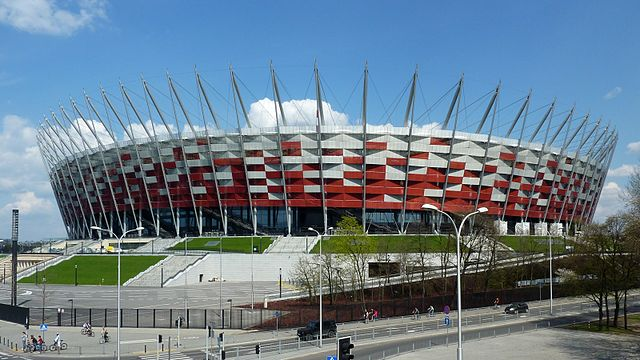
\includegraphics[scale=0.5]{stadion.jpg}
			%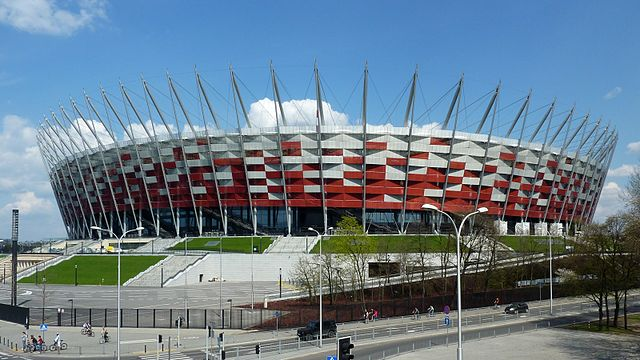
\includegraphics[scale=0.5,bb=0 0 30 30]{stadion.jpg}
			\end{center}
		\end{figure}
	\end{frame}

\end{document}
